\section{Where an intervention appears to act}\label{sec:claim3}

\begin{figure*}[t]
  \centering
  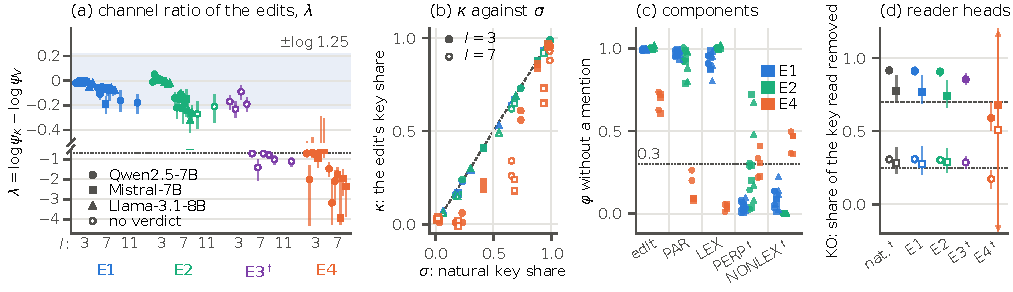
\includegraphics[width=\textwidth]{figures/fig_law.pdf}
  \caption{\textbf{The preregistered channel-ratio law failed.} Qwen2.5-7B, Mistral-7B and Llama-3.1-8B, 80 stories. (a)~$\lambda = \log\psi_K - \log\psi_V$ per edit family (E1, E2: steering vectors from held-out stories and from unrelated sentences; E3: features of a public sparse autoencoder; E4: a remap trained at the writing token), depth and format, with 90\,\% intervals and the $\pm\log 1.25$ band; hollow: no verdict (E3's gate failed; values recomputed). (b)~$\kappa$, the edit's key share, against $\sigma$, the natural key share at the same depth and format (descriptive). (c)~Identity effect without a mention of each edit's component along the natural write (PAR), along the English lexical span (LEX) and orthogonal to each. (d)~Share of the key read removed by blocking the reader heads, per family, beside the natural write; open: random head sets, which the natural write also fails to keep under the preregistered 0.25.}
  \label{fig:law}
\end{figure*}

\textbf{Which cache channel an intervention appears to act through depends on the prompt and on the edit; a preregistered law that would have predicted it from the model's own read failed.}

\paragraph{A motivating case.}
The released remap of \citet{anonymous2026fitted} is a rank-16 distributed alignment search subspace \citep{geiger2024finding} at the output of block 4 over the move event, trained so that the model answers a fixed permutation of the source location. With \fmtOpt{}, a key-only exchange at the writing token attributes part of its effect, beyond a PCA control, to the keys, as we reproduce (\cref{app:remap}). Changing only the format barely changes its behavioural effect, yet the channel that appears to carry it flips: at Qwen2.5-72B its keys carry \psiLetterQwen{} of the effect with lettered options and \psiNoneQwen{} without a later mention, its values the reverse (discovery sample; likewise for a refit without later mentions).

\paragraph{The law and its test.}
We preregistered a law that extends the \emph{format law} of \cref{sec:claim1} from the model's own read to edits: an edit written at the writing token at depth $l$ is read through key and value in the model's own ratio at that depth and format. With $\psi_C$ the edit's identity effect through channel $C$ as a share of the natural write's, from block $l{+}1$ on,
\begin{equation}\label{eq:lambda}
\lambda = \log\left(\psi_K/\psi_V\right),
\end{equation}
and the law holds in a cell when the 90\,\% interval of $\lambda$ lies inside $\pm\log 1.25$. An edit at the writing token reaches later tokens only through its keys and values, and as the runs differ only there, writing the source run's residual is the natural clamp itself: our equivalence control. Rows with the key moved halfway were classified as departures (\cref{app:law}). Five families were tested, in up to three models, four depths and four formats: steering vectors from held-out stories or unrelated sentences \citep{turner2023actadd,panickssery2023caa}; features of a public sparse autoencoder \citep{bussmann2024batchtopk,andyrdt2025saes}; a rank-16 remap trained at the writing token with the released training code of \citet{anonymous2026fitted}; and \emph{non-lexical} steering vectors, which write the value in another language, as a synonym, or without its English lexical component (\cref{app:edits}).

\paragraph{The outcome.}
Even steering vectors close to the natural edit depart from the natural channel ratio; the format law describes the model's own written value and does not predict how an edit is attributed. In the preregistered core test the steering vectors' departures are small but graded ($\bar\lambda$ = $\JcOnePoolEoneMistralSeven$ to $\JcOnePoolEtwoMistralSeven$; every pooled value inside the margin, not every statistic): the format law does not transfer to edits as a channel-ratio law (did not hold; in Llama-3.1-8B for the vectors from unrelated sentences too; \cref{fig:law}a,~b). At the shallowest depth every statistic is equivalent ($|\lambda| \leq \JcOneLamThreeAbsMax$; exploratory); deeper, the keys under-read the steering vectors, pooled by 4.5--12\,\% ($\bar\lambda$ $\JcTwoPoolEoneLlamaEight$ to $\JcTwoPoolEtwoLlamaEight$), % verbatim: outcome J part C
and every failing statistic sits in a cell with a small natural key read (\JcOneNeIDKMin--\JcOneNeIDKMax{} nats; post hoc).

\paragraph{Edits far from the natural write.}
Edits that change the value through a learned remap are read mainly through the value ($\bar\lambda$ = $\JcFourPoolEfourQwenSeven$ / $\JcFourPoolEfourMistralSeven$): the key channel does not read them as it reads the written word (risky; did not hold). Its size depends on depth (under \fmtPost{} at block 7, $\psi_K$ \JcFourPsiKWpostSevenQwenSeven{} against $\psi_V$ \JcFourPsiVWpostSevenQwenSeven{} at Qwen2.5-7B; post hoc). The autoencoder test was not evaluable: its gate scored positions that the dictionary's published fit excludes. Identity-carrying components orthogonal to the natural write or to the lexical span are also read mainly through the value (risky; did not hold; \cref{fig:law}c). The non-lexical steering vectors are read less through the key, but write far from the natural state: the predicted lexical boundary was not isolated, so we claim neither that the token-form account holds for edits nor that it is contradicted (risky; did not hold). The reader heads read the steering vectors like the natural value, but the test failed on a random-set control that the natural value also fails (did not hold; post hoc reading), and it was not evaluable for the autoencoder and the remap (failed gate; small key read; \cref{fig:law}d, \cref{app:lawresults}).

\paragraph{Post hoc: distance from the natural write.}
Post hoc, the departures follow how far an edit's cached keys and values lie from the natural ones ($\nu$, a relative distance): of the $\lambda$ statistics of identity-carrying edits, \JcNuEqLow{} of \JcNuNLow{} with $\nu < 0.1$ are equivalent, \JcNuEqMid{} of \JcNuNMid{} with $\nu$ between 0.1 and 0.3, and \JcNuEqHigh{} of \JcNuNHigh{} beyond (Spearman $\JcNuRhoNu$; \cref{app:nu}). $\nu$ is collinear with the key cosine, so which matters is open. Rule: report an intervention's channel only beside the model's own read at the same depth, in more than one prompt, and with the edit's distance from the natural write.

\paragraph{The binding swap of \citet{prakash2025lookbacks}.}
At block 28 of Qwen2.5-14B an identity edit is copy-read like the natural value ($\kappa \leq 0.30$), while the binding swap there is key-read; key-flat reading is not a property of depth for identity edits ($\kappa$ \JcSixKappaCaaNoMention{} against \JcSixKappaBindNoMention{} without a mention). This does not separate kind from depth, because the natural read there is itself copy-only, and the swap changes no answer in two of the three formats. Binding forms only after the identity key route closes in every model screened, so a binding swap cannot be compared with an identity edit at a depth where the key route is open (risky; held; a prediction for such a window was not evaluable); the four earlier preregistered predictions on this swap, which failed, stand (\cref{app:binding}).
